%%%%%%%%%%%%%%%%%%%%%%%%%%%%%%%%%%%%%%%%%%%%%%%%%%%%%%%%%%%%%%%%%%%%%
%
% CSCI 1430 Writeup Template
%
% This is a LaTeX document. LaTeX is a markup language for producing
% documents. Your task is to fill out this
% document, then to compile this into a PDF document.
% You will then upload this PDF to `Gradescope' - the grading system

\documentclass[11pt]{article}

\usepackage{amsmath}

\usepackage{braket}
\usepackage[english]{babel}
\usepackage[utf8]{inputenc}
\usepackage[colorlinks = true,
linkcolor = blue,
urlcolor  = blue]{hyperref}
\usepackage[a4paper,margin=1.5in]{geometry}
\usepackage{stackengine,graphicx}
\usepackage{fancyhdr}
\setlength{\headheight}{15pt}
\usepackage{microtype}
\usepackage{times}
\usepackage{booktabs}


\frenchspacing
\setlength{\parindent}{0cm} % Default is 15pt.
\setlength{\parskip}{0.3cm plus1mm minus1mm}
{\normalsize {\tiny }}
\pagestyle{fancy}
\fancyhf{}
\lhead{QC mentorship program}
\rfoot{\thepage}

\date{}

\title{\vspace{-1cm}Finding the lowest eigenvalue of a Hamiltonian Using Variation Quantum Eigensolver (VQE)}

\usepackage{listings}
\usepackage{color}

\definecolor{codegreen}{rgb}{0,0.6,0}
\definecolor{codegray}{rgb}{0.5,0.5,0.5}
\definecolor{codepurple}{rgb}{0.58,0,0.82}

\lstdefinestyle{mystyle}{
	commentstyle=\color{codegreen},
	keywordstyle=\color{magenta},
	numberstyle=\tiny\color{codegray},
	stringstyle=\color{codepurple},
	basicstyle=\footnotesize,
	breakatwhitespace=false,
	breaklines=true,
	captionpos=b,
	keepspaces=true,
	numbers=left,
	numbersep=5pt,
	showspaces=false,
	showstringspaces=false,
	showtabs=false,
	tabsize=2
}

\lstset{style=mystyle, language=python , frame=single}

\begin{document}
	
	\maketitle	
	
	\vspace{-3cm}
	\thispagestyle{fancy}
	
	
	\section*{Definitions}
	
	
	{\addtolength{\leftskip}{7mm}
		
		
	Let's start by defining some definitions that we will use later in this document:
	
	- \textbf{Hamiltonian}:\\
	{\addtolength{\leftskip}{7mm} 
	A Hamiltonian is an operator that describes the sum of kinetic and potential energies in a given system. Here is an expression of a the Hamiltonian: 
	$\displaystyle {\hat{H}}={\hat{T}}+{\hat{V}}$\\
	where $\hat{T}$ represent the operator of the kinetic energy and $\hat{V}$ represent the operator of the potential energy.
	}\\
	
	- \textbf{Eigenstate}\\
	{\addtolength{\leftskip}{7mm}
	A state represent a possible energy state of the system. For example, if we have a Hydrogen atom, a possible state is to have the electron in the first orbital, and because this is the lowest energy state this atom can have, we call this state the "ground state". we can represent any state using the bra-ket notation $\ket{\psi}$ which can be any possible energy state of the system. what make an Eigenstate different from other states is that it we can represent any state using combination of the eigenstates.\\\\
	An important note about eigenstates:\\\\
	$\langle A| = {\begin{pmatrix}A_{1}^{*}&A_{2}^{*}&\cdots &A_{N}^{*}\end{pmatrix}}$\\
	$\langle A|^{\dagger }=|A\rangle$\\\\
	So we can use this $\langle A|H|A \rangle$ to get the energy of that state $A$
	}\\
	
	- \textbf{Eigenvalue}\\
	{\addtolength{\leftskip}{7mm}
	Each Eigenvalue represents the quantity or the weight of contribution the corresponding Eigenstate to the current state of the system. $\lambda$ represents the Eigenvalue.
	}\\

	- \textbf{Pauli matrices}
	Those are some 2 x 2 complex matrices, which act as building blocks or the basis of our 2 x 2 Hamiltonian. so we will try to decompose our given Hamiltonian later in our problem to a linear combination of Pauli matrices, or their tensor product, if there is more than one qubit. Here are the basis:
	
	${\begin{aligned}\sigma _{1}=\sigma _{x}&={\begin{pmatrix}0&1\\1&0\end{pmatrix}}\\\sigma _{2}=\sigma _{y}&={\begin{pmatrix}0&-i\\i&0\end{pmatrix}}\\\sigma _{3}=\sigma _{z}&={\begin{pmatrix}1&0\\0&-1\end{pmatrix}}\,.\end{aligned}}$
	
	alongside with the identity matrix which we can call $\sigma_{0}$\\
	
	
	- \textbf{Ansatz}\\
	In our problem: we need to find the ground state of a system, so we need to explore all possible states or as wide spectrum of states as we can. The Ansatz are circuits composed of gates with parameter. we use and change those parameters till we find the ground state. For example
	
	
	 

   	}
	
	
	\section*{Problem Statement}
	{\addtolength{\leftskip}{7mm}
		In this task we are given a Hamiltonian of a system and we are asked to find the ground state of that Hamiltonian.
		
		\begin{equation*}
		H = 
		\begin{bmatrix}
		0 & 0 & 0 & 0\\
		0 & -1 & 1 & 0 \\
		0 & 1 & -1 & 0 \\
		0 & 0 & 0 & 0\\
		\end{bmatrix}
		\end{equation*}
		
	}



	\section*{Procedure}
	{\addtolength{\leftskip}{7mm}
		\section*{2D solution}
			{\addtolength{\leftskip}{7mm}
			First Solution is to simplify our Hamiltonian into 2D problem instead of 4D, because we observed that all values are 0 except the inner 2 x 2 matrix.
			now our Hamiltonian is this:
			\begin{equation*}
			H = 
			\begin{bmatrix}
			-1 & 1\\
			1 & -1
			\end{bmatrix}
			\end{equation*}
			
			now we will try to decompose this into a combination of Pauli operators. It will be like this H = $\sigma_{x} - I$
			
			Then we will use our Ansatz -in this case we will use $RYRY$- the first $RY$ is rotating the x by -$\frac{\pi}{2}$ and the second $RY$ is parameterized by $\theta$ to span all possible real values
			
			Now we will use the fact that $\langle \psi|H|\psi \rangle = \langle \psi|H_{1} + H_{2} + ...... + H_{i}|\psi \rangle$ where $H_{i}$ is the Pauli operators and then we can use the fact that $\langle \psi| H_{i} | \psi \rangle$ represent the expected value of $H_{i}$ which can be known by measuring the $|\psi \rangle$ and then average the results. we will do this on all possible $\theta$s  till we find the lowest energy (lowest eigenvalue) and the corresponding eigenstate
			
				
		}
	}


	\section*{Results}
	
	As we mentioned before in the 2D solution we will just find the lowest energy along different $\theta$s and here is a graph showing Expectation value vs $\theta$\\
	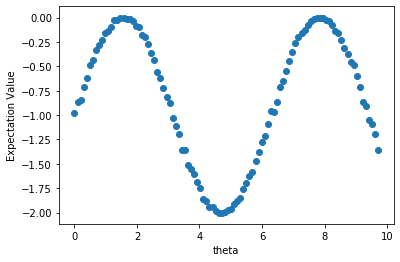
\includegraphics[scale=1]{../download}
	
	
	
	\section*{References}
	1- \href{https://www.mustythoughts.com/post/variational-quantum-eigensolver-explained}{Variational Quantum Eigensolver explained Article by Michał Stęchły} (It has been an inspiration of how to write a simple, rich, and easily understandable article and some of the examples are from that article)
	
	2- Wiki notes
	
	
	
\end{document}
